% Koma-Script Basisklasse
\documentclass[a4paper,12pt,pagesize,headsepline,bibtotoc,titlepage,abstracton]{scrartcl}

\usepackage[utf8]{inputenc}		% direkte Eingabe von Umlauten & Co. (Vorsicht: Encoding im Editor muss auch UTF-8 sein!)

\usepackage[T1]{fontenc}			% T1-Schriften

\usepackage{mathptmx}			% Times/Mathe \rmdefault
\usepackage[scaled=.90]{helvet}	% Skalierte Helvetica \sfdefault
\usepackage{courier}			% Courier \ttdefault

% Zusatzpakete für mehr mathematische Symbole, Einfügen von Grafiken 
% und bessere Bildunterschriften
\usepackage{amsmath,amsthm,amsfonts,graphicx,caption}

% Wenn man direkt mit dem pdflatex eine PDF-Datei erzeugt, sollten diese beiden Pakete eingebunden werden
\usepackage{hyperref} % Hyperlinks anklickbar
\usepackage{ae,aecompl} % bessere Bildschirmschriftarten usw.
\usepackage{epstopdf} % support eps 
\usepackage{subcaption}
\pagestyle{headings}

% Abstand der Kopfzeile vom Text:
\headsep4mm

\typearea[current]{current}     % Satzspiegel neu berechnen

% andere Bildunterschrift mit Hilfe von caption
\renewcommand{\figurename}{Fig.}
\renewcommand{\captionlabelfont}{\bf}

\newcommand{\quot}[1]{{``#1''}}

\usepackage{color}

\title{
	\includegraphics*[width=0.4\textwidth]{hpi_logo_2017.eps}\\
	\vspace{24pt}
	Genetic Doodle Jump
}
\subtitle{
	Seminar\\
	Machine Intelligence with Deep Learning\\
	Fall Semester 2017/2018
}
\author{
	Marcel Jankrift\\
	Fabian Sommer\\
	Toni Stachewicz\\[12pt]
	Supervisor:\\
	Goncalo Mordido,
	Dr. Haojin Yang\\
	Prof. Dr. Christoph Meinel
}
\date{\today}

\begin{document}
\maketitle
\tableofcontents

\newpage

\begin{abstract}
Games usually have a wide range of possible parameters to tune. Often times, simple neural networks can meet all the requirements and perform well. However, training the net often takes many hours or a few days. The training time can be reduced tremendously by using neural nets in combination with a genetic algorithm. In this paper we present how we applied a deep genetic algorithm on the game \quot{Doodle Jump}. We especially pay attention to the configuration of the genetic algorithm, describe the undertaken changes and show, which influence they have on the performance.
\vskip 0.7cm
\noindent \textbf{Keywords.} Deep Learning, Genetic Algorithm, Artificial Intelligence, Games
\end{abstract}
\newpage

\section{Introduction}
Teaching an AI to play a simple game has become an interesting research topic in the last couple of years. AlphaGo\footnote{\url{https://deepmind.com/research/alphago/}} by Google Deepmind is probably the most famous example of computers playing games. The algorithm plays the board game Go, whose complexity is orders of magnitude higher than the complexity of chess. In a tournament against Lee Sedol (one of the world's best Go player) in 2016 the AI won four out of five games.

We did something similar in our research seminar, but with a less complex game: Doodle Jump. The player of this video game has to jump on randomly located platforms in order to get higher and thus, get a higher score. In our approach we use a genetic algorithm in combination with neural networks ??/for the machine learning part. An artificial neural net (ANN) is a machine learning algorithm inspired by nature. It consists of neurons, which calculate an output based on an input similar to a biological nerve cell. Those neurons are connected with each other to enable an information flow within the network. In order to improve the performance of an ANN, many parameters --- for example the biases of the neurons or the weight of connections --- can be tuned.

At this point we make use of the genetic algorithm. This algorithm is modelled on biological evolution. There are many individuals which form a population. Applied to our implementation, those are the different neural nets playing the game. After all players died, we select the best of them and perform crossover and mutation like in nature on those. Hence, we create a new generation, which is supposed to be better than the previous one. In this way, we always create better and better neural networks.

In the next two sections, we introduce the basics of the Doodle Jump game in detail and give a rough overview of our user interface. After that, we pay special attention to the used neural network. In section \ref{sec:ga} we present our genetic algorithm, in particular with focus on the basic operations of this algorithm and its evalution. Finally, we conclude our work and show some interesting findings.

\section{Doodle Jump}
\subsection{Original game}

The video game Doodle Jump is developed for mobile devices by Lima Sky\footnote{\url{http://www.limasky.com/}}. The player --- the so called \quot{doodler} --- has to jump on platforms in order to get a higher score. There are four different types of platforms:
\begin{enumerate}
    \item Regular ones, which neither move nor break
    \item Horizontally moving platforms
    \item Vertically moving platforms
    \item Vanishable ones, which disappear after jumping on it once
    \item Breaking platforms, where the doodler can not jump on
\end{enumerate}
The platforms are pseudo randomly located on the map. Pseudo randomly located means, that there will always be at least one platform, which is reachable from the previous one and non-breakable (See Fig. \ref{abb:doodlejumpgame}). In other words, there is always a way to reach an infinite score. However, the higher the achieved score, the more difficult the game becomes. The difficulty is reached via higher distances between the platforms and the increased usage of moving and vanishable platforms.

The game also includes bonus features, such as propeller hats, jetpacks, rockets, springs or trampolines. These allow the player to jump higher and faster and therefore skip some platforms. Indeed, there are also \quot{enemies} in the game for example monsters, UFOs or black holes. If the doodler hits a monster or comes close to a black hole or UFO, it dies and the game is over. Monsters and UFOs can also be killed by shooting or jumping on them.

To control the doodler the player of the game has to tilt his mobile devices left and right. If the doodler hits the left or right boundary of the game, it will appear on each other's side. Shooting is performed by tapping on the screen. The downrange depends on the tapping position. Once a player falls down and hits the bottom the game is over.

\begin{figure}[h]
\begin{center}
\includegraphics*[width=0.4\textwidth]{images/game}\\
\caption{Screenshot of original Doodle Jump game}
\label{abb:doodlejumpgame}
\end{center}
\end{figure}

\subsection{Simplified implementation}

Since we do not want to perform the deep learning part on a mobile device or within an emulator, we decided to use an implementation, which runs in a browser. We are using \quot{HTML5 Doodle Jump} by ntcnet83\footnote{\url{https://github.com/ntcnet83/html5-doodle-jump}}, which we found on github\footnote{\url{https://github.com/}}. This custom version of the is written in HTML5 and JavaScript. The doodler can be control via left and right arrow keys. In contrast to the original implementation, this version of the game contains less features, which makes the game simpler at the end:
\begin{itemize}
\item Except springs, there are no other bonuses.
\item There are no enemies. Hence, the only way to die is falling down.
\item The feature shooting is not necessary and therefore not available.
\item The game does not have vertically moving platforms.
\item The difficulty changes after a certain score, but only through the usage of more moving and vanishable platforms. The distances between the platforms stay the same.
\end{itemize}

Our machine learning part runs in the browser as well. We use the \textit{Synaptic} library\footnote{\url{https://github.com/cazala/synaptic}} in order to create our neural networks. This library provides a high level interface to simply initialize a perceptron. Furthermore, adapted the genetic algorithm implemented in the \textit{Genetic.js} library\footnote{\url{https://github.com/subprotocol/genetic-js}}. Both libraries are written in JavaScript.


\section{User Interface}

\section{Network Layout}

\section{Genetic algorithm}
\label{sec:ga}

Whether or not the neural network performs well at playing the game very heavily depends on the specific parameters it uses: Each node possesses a bias and each edge has a weight. Even though the network is rather small, there are too many weights and biases to optimize them manually. 

We therefore employ a genetic algorithm to obtain good parameters for the network. At any time, there is a number of different networks, so-called candidates, all playing the game independent of each other. Once they are all done, their performance is evaluated using a fitness function. The best candidates are then selected and combined in different ways to obtain the next generation of candidates. This combination process is called crossover. Finally, some parameters of some candidates are altered (mutated) to make it possible to generate any network. This new generation is then evaluated again, and the process is iterated.

Doodle Jump is a game where each level is generated randomly. We want to end up with a network that is able to play any level well, regardless of the specific generated layout. The performance of any one network on any specific level may not necessarily be indicative of the networks ability to play the game overall. Therefore, each network plays several levels simultaneously, and each level is taken into account when evaluating the performance.

In order to make the performance of different candidates comparable, all candidates of a generation play the same set of levels. However, for each generation a new set of levels is generated. Otherwise, we might end up with a network that excels in playing the specific set of levels used for evaluation but fails at any other level. Therefore, we can avoid overfitting.

We want to choose the different parts of the genetic algorithm so that the learning process is as quick as possible, i.e. the average score achieved by the candidates after 100 generations should be as high as possible.

\subsection{Fitness function}

The fitness function measures the ability of the candidates to play the game well. Doodle Jump already provides a score which measures the height a player achieves. Since the games aim is to maximize that score, we used the score as initial fitness function.

Beyond that, there are many other fitness function one could think of. For example, at the very beginning of the optimization process, many candidates might do nothing at all, while others move a little bit into the direction of the next platform, but not far enough to actually land on it. All candidates would thus achieve a score of zero, and the primitive fitness function would be unable to discriminate between them. Another fitness function, which rewards candidates that got closer to the platform they failed to jump on might speed up the learning process in the first few generations. It would also be helpful later on, when different candidates might fail at the same platform, thus achieving an equal score. However, such a fitness function would include prior knowledge about how to play the game well. We want to avoid using such fitness functions, since for other problems, prior knowledge might not be available, or might not lead to the optimal solution if available. 

One measurement that does not involve any prior knowledge is time. Between two candidates, both achieving similar score, where one jumps once on every platform and the other has to jump twice on every platform before attempting the next jump, we want to prefer the first candidate since he is climbing twice as fast. Therefore, the required time should negatively affect the fitness of candidates.

We tested multiple fitness functions achieving this in different ways:
\begin{itemize}
\item $fitness_1 = score$
\item $fitness_2 = \frac{score}{time}$
\item $fitness_3 = score - time$
\item $fitness_4 = normalized(score - time)$
\item $fitness_5 = score^2 - time$
\item $fitness_6 = normalized(score^2 - time)$
\end{itemize}

For each fitness function, we monitored the learning process for the first 100 generations. Since it is a random process with a high variance, we repeated this 10 times for each function. Figure \ref{fig:fitness} shows the evaluation results. 

\begin{figure}[hbp]
\begin{center}
\begin{subfigure}[b]{0.45\textwidth}
    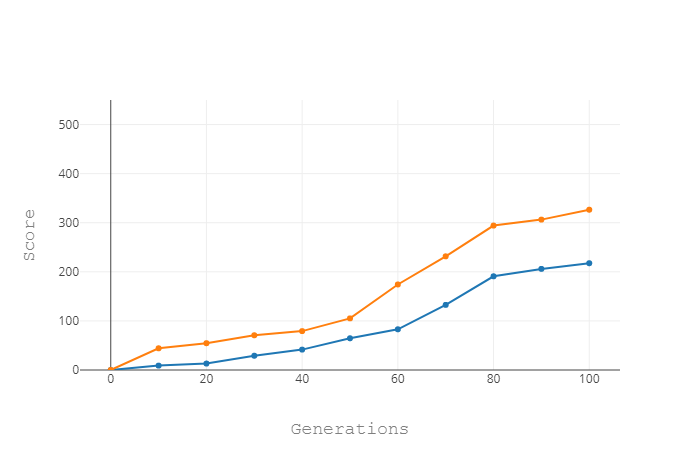
\includegraphics[width=\textwidth]{images/score.png}
    \caption{$score$}
\end{subfigure}
\begin{subfigure}[b]{0.45\textwidth}
    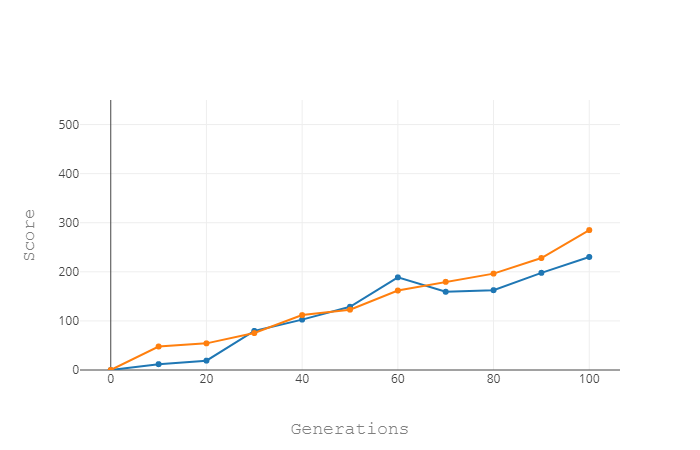
\includegraphics[width=\textwidth]{images/scoredivtime.png}
    \caption{$\frac{score}{time}$}
\end{subfigure}
\begin{subfigure}[b]{0.45\textwidth}
    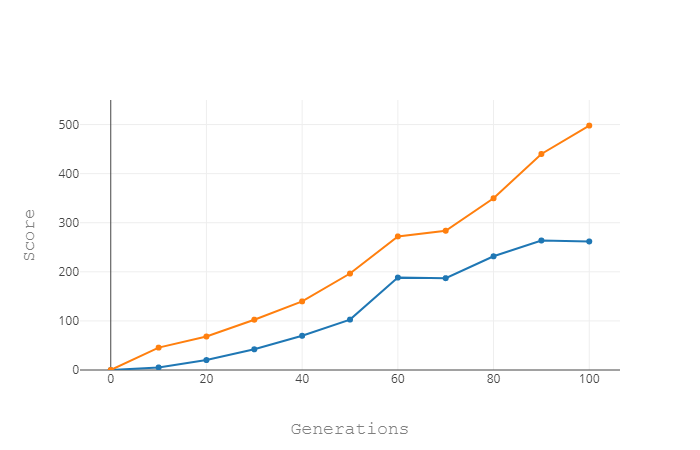
\includegraphics[width=\textwidth]{images/scoreminustime.png}
    \caption{$score - time$}
\end{subfigure}
\begin{subfigure}[b]{0.45\textwidth}
    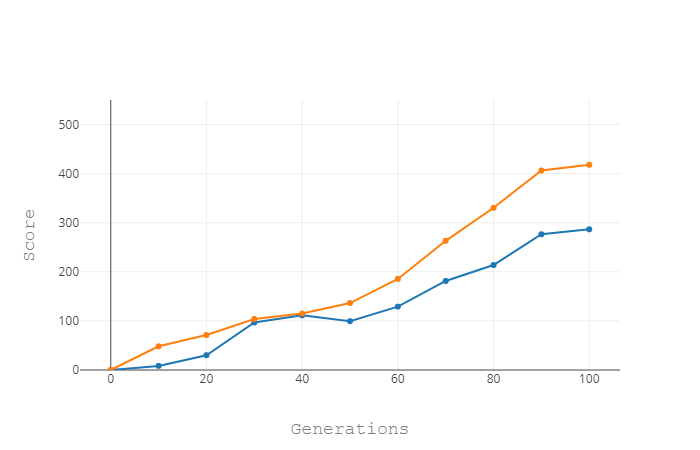
\includegraphics[width=\textwidth]{images/normscoreminustime.png}
    \caption{$norm(score - time)$}
\end{subfigure}
\begin{subfigure}[b]{0.45\textwidth}
    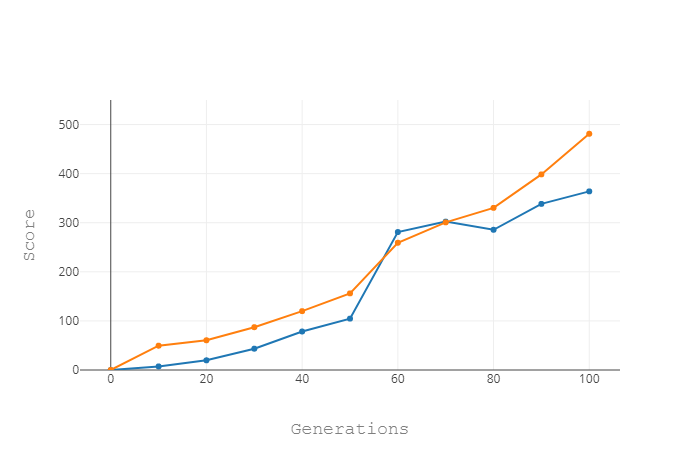
\includegraphics[width=\textwidth]{images/scoresquared.png}
    \caption{$score^2 - time$}
\end{subfigure}
\begin{subfigure}[b]{0.45\textwidth}
    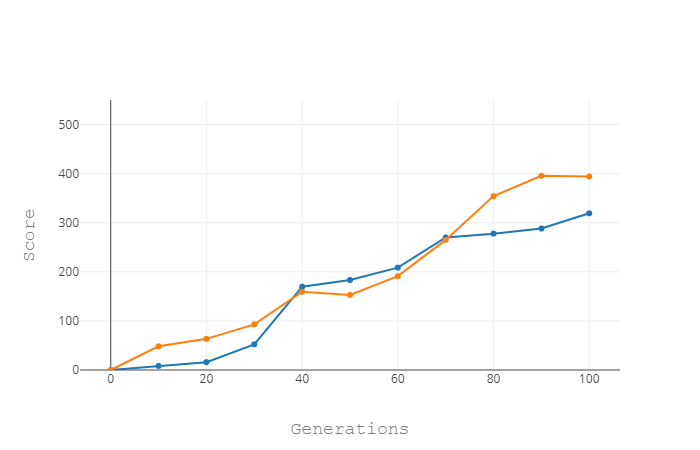
\includegraphics[width=\textwidth]{images/normscoresquared.png}
    \caption{$norm(score^2 - time)$}
\end{subfigure}
\caption{Evaluation of different fitness functions. On the x-axis are the number of generations, on the y-axis the average score (red curve) and its standard deviation (blue).}
\label{fig:fitness}
\end{center}
\end{figure}

All functions lead to a learning where to expected score is rising close to linearly. Score divided by time leads to the slowest leaning, since it essentially just measures the (nearly constant) speed in which any candidate is traveling upwards, so the fitness is nearly constant as well. All other functions involving time perform better than just taking the score. $fitness_3$ is one of the simplest ways of rewarding for gained score while penalizing for taken time, whereas $fitness_5$ puts emphasis on score and only uses time to break ties between two candidates that obtained the same score. 

Each candidate is playing multiple levels at once, at the fitness calculated for each level is averaged to obtain the fitness for the candidate. Consider two levels such that one of them is very easy and a high score is easily obtained and the other is very hard, where only a few candidates might get beyond the first platform. In that case, the average for both $fitness_3$ and especially $fitness_5$ is dominated by the performance of each candidate on the easy level, since it yields far more score compared to the hard level. If we want to put equal weight on each level regardless of difficulty, this can be achieved by normalizing the fitness for each level, and then taking the average. However, our tests show that, at least in the first 100 generations, this merely slightly slows down the learning process. Ultimately, $fitness_3$ turns out to be the best of the tested functions, featuring both a high average score after 100 generations and a high consistency, the standard deviation of the score being only about half the average score.

\subsection{Selection and Crossover}

After the fitness of each candidate has been determined, the $n$ top candidates are selected to generate offspring that form the next generation. Here, $n$ is a parameter that can either be chosen or dynamically adapted during the algorithm. Choosing a higher $n$ leads to more diverse offspring and the possibility to find small local optima that might not be found otherwise, but as their parents are worse, usually they can be expected to be worse as well.

The crossover serves to combine two different candidates into a new, different candidate who inherits traits of both of them, much like two individuals having a child together. Our candidates are defined by two different traits: Their node biases and their edge weights. For the crossover, we order all nodes and choose a random cutoff point. All the child's nodes before the cutoff point take the bias of the corresponding node of the first parent, the rest gets the biases of the second parent. One parent is selected randomly and all edge weights are copied from it.

We chose to select the best $n=4$ candidates as parents. The next generation consists of:

\begin{itemize}
\item All the parents, as they were before.
\item One child made from the two best parents which is then mutated.
\item Two parents that are chosen randomly and independent from each other, which are then mutated.
\item For all remaining nine candidates, two random parents are chosen, they are crossed over and the resulting child is mutated.
\end{itemize}

Therefore, we achieve a good diversity between the candidates while still maintaining a high quality in the offspring.

\subsection{Mutation}
\subsection{Retaining best candidates}

After all games died with one generation we select the top players of this run and reuse them without any modification in the next generation. The amount of retained candidates depends on the performance of the current run compared with the previous one. However, the number of players kept is limited to the range of three to five out of sixteen. The reason, why we have such a complex algorithm is, that we want to a high amount of good players and throw away a large number of bad ones. In order to explain it in detail we use an example which is depicted in graphic \ref{abb:retaining}. It shows the players of three generations sorted by fitness.

In the first generation we keep all top five players, since we can not compare them to another run. The only requirement is that the best player has a fitness of more than 0. Otherwise, we throw away the whole population due to the bad score.

The second generation performs a little worse than the previous one. Hence, we will keep less candidates. First, we compare the top five players with the previous run. In this concrete example only two players are better than the last best five. We then also select the third player, because this is the minimum number of retained candidates. The main idea behind this lower limit is, that we do not want to throw away to many information.

After the next run we compare the best players again. Since we always focus on the best five players, the number of reused candidates --- which us four now --- can increase again. That would not be the case, if we only compare the individuals with the previously retained ones. If we did that, we would have three bots and would stay at this number forever.

\begin{figure}[h]
\begin{center}
\includegraphics*[width=0.8\textwidth]{images/retain_candidates}\\
\caption{Example of retained candidates}
\label{abb:retaining}
\end{center}
\end{figure}



\section{Implementation details}
\subsection{Disabling passing through walls}

Initially when we started working on the project, there existed a huge local optimum where candidates that would choose to accelerate to the right (or left) constantly would quickly go so fast that they were able to hit a good number of platforms before falling down, therefore easily beating any initial candidates that tried to work with the input data in any way. This behavior did not resemble how a human would approach the game, nor was it visually appealing. It also was not a sophisticated strategy (as any information about the surroundings of the doodler would just be discarded) and had a rather low ceiling in terms of how many points could be achieved that way.

In order to counteract this, we decided to modify the game in a way that any player touching the walls would die, instead of reappearing on the other side of the level. This lead to an interesting effect in combination with the third fitness function, $score - time$. Score is awarded only if at least one platform is being reached. Time, on the other hand, starts counting immediately. Therefore, a candidate that would slowly move into the direction of the first platform, but not fast enough to reach it before he would die, would get a negative fitness. Another candidate that always goes right, therefore hitting the right wall as soon as possible, also gets a negative fitness, but due to the speed of his suicide, he still gets a better fitness than the first candidate. Ultimately, after a few generations, all candidates had learn to commit suicide as quickly as possible. We could resolve this problem by treating every negative fitness as equal.

In the end, we re-enabled passing through the wall, but limited the maximum speed the doodler could achieve, so that constantly accelerating in one direction was no longer a viable strategy.

\subsection{Dealing with moving platforms}
\subsection{Dealing with fake platforms}
\subsection{Dealing with springs}
\section{Conclusion and Future Work}

\newpage
%%%% bibtex file %%%%%%
\bibliographystyle{alphadin}
\bibliography{references} 

\end{document}